\documentclass[12pt]{article}
\usepackage[a4paper, total={6in, 8.5in}]{geometry}
\usepackage{graphicx}
\graphicspath{ {images/output/} }
\usepackage{amsmath}
\usepackage{minted}
\usepackage{multicol}
\usepackage{caption}
\usepackage[english]{babel}
\usepackage{placeins}
\usepackage{titling}


\begin{document}

\vspace*{\fill}
\begin{center}

    \emph{Heaven's Light is Our Guide} \\
    \textbf{Rajshahi University of Engineering and Technology} \\

    \begin{figure}[H]
        \centering
        
\includegraphics[scale=.34]{images/RUET_logo.png}
        \label{fig:ruet_logo}
    \end{figure}
    \vspace{5mm}

    \textbf{Course Code}\\
    ECE 2214\\
    \vspace{3mm}
    \textbf{Course Title}\\
    Numerical Methods and Discrete Mathematics Sessional

    \vspace{5mm}
    \textbf{Experiment Date:} {November 18, 2023},\\
    \textbf{Submission Date:} {December 2, 2023}\\

    \vspace{5mm}
    \textbf{Lab Report 10:} Implementing Secant method of root finding in MATLAB.

    \vspace{15mm}

    \begin{tabular}{c|c}
        \textbf{Submitted to} & \textbf{Submitted by} \\
        Md. Omaer Faruq Goni  & Md. Tajim An Noor     \\
        Lecturer              & Roll: 2010025         \\
        Dept of ECE, Ruet     &                       \\
    \end{tabular}

\end{center}
\vspace*{\fill}


\pagebreak
\clearpage
\title{Finding root of nonlinear equation using Secant Method.}
\author{}
\date{}
\maketitle

\section*{Introduction}
\subsection*{Secant Method}
Secant Method is open method and starts with two initial guesses for finding real root of non-linear equations.
In Secant method if $x_0$ and $x_1$ are initial guesses then next approximated root $x2$ is obtained by following formula:\cite{sec}
\[x_2 = x_1 - \frac{(x_1-x_0) \times f(x_1) }{f(x_1) - f(x_0)}\]
This method is similar to the false position method, except in false position method we bracket the root with initial guesses. But in secant method its not necessary. Also in false position method, we need to change the $x$ intersect after checking its value for the function but in secant method we just need to change only one of the guesses until we reach our requirement for the result.



\section*{Tools Used}
\begin{itemize}
    \item MATLAB R2021a - for writing and running code.
    \item MacTeX -\LaTeX  compiler.
    \item VS Code with \LaTeX workshop extension as a text editor.
\end{itemize}

\section*{Process}
\subsection*{Code for Secant Method:}
•	File 1 – Function file
\begin{minted}[breaklines, linenos]{matlab}
function secant_func(eqn, a, b, error)
    syms x;
    
    fa = eval(subs(eqn, x, a));
    fb = eval(subs(eqn, x, b));
 
    c = b- fb*(b-a)/(fb-fa);
    fc = eval(subs(eqn, x, c));
 
    while abs(fc) > error
       arr = [a b c fc];
       disp(arr);
       a = b;
       fa = fb;
       b = c; 
       fb = fc;
       c = b- fb*(b-a)/(fb-fa);
       fc = eval(subs(eqn, x, c));
    end

          arr = [a b c fc];
    disp(arr);

    disp("The root(approx..) is: ");
    disp(c);
end
\end{minted}
•	File 2 – Main file
\begin{minted}[breaklines, linenos]{matlab}
clc, clear all, close all;
syms x;
 
eqn = input("Enter equation: ");
a = input("First guess: ");
b = input("Second guess: ");
error = input("Error: ");
 
secant_func(eqn, a, b, error);
\end{minted}
\subsection*{Output}
\begin{center}
    \centering
    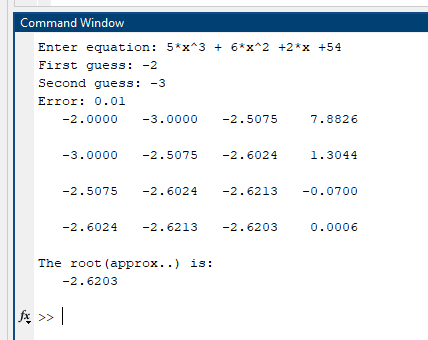
\includegraphics[width = .9\textwidth]{image.png}
    \captionof{figure}{Secant method.}
\end{center}




\section*{Functions}
All of the functions used in this experiment was used in the previous experiments. Only addition is how the user defined function in declared:
\begin{minted}{matlab}
function secant_func(eqn, a, b, error)
\end{minted}
Here \emph{function} is a keyword to define a function. In this case the function is named \emph{secant\_func} and it takes 4 inputs; the equation \emph{eqn}, the first guess \emph{a}, the second guess \emph{b} \& the error margin \emph{error}.\\
When this function is called in the main file, it's given the four parameters and then is executes.
\pagebreak
\bibliographystyle{IEEEtran}
\bibliography{ref}

\end{document}
